\documentclass{beamer}

\usepackage{beamerthemeHannover,graphics,amsmath,bm}

\title[Measurement Invariance]{Tests for Measurement Invariance when Subgroups are Unknown}
\author{Ed Merkle\inst{1} \and Achim Zeileis\inst{2}}
\institute{\inst{1} University of Missouri \and \inst{2} Universit\"{a}t Innsbruck}
\date{Supported by grant SES-1061334 from the National
  Science Foundation}

\begin{document}

\frame{\titlepage}

\frame{
  \frametitle{}
  \tableofcontents}


\section{Background}
% Define measurement invariance
\frame{
  \frametitle{Measurement Invariance}
  \begin{itemize}
    \item Measurement invariance: Sets of tests/items consistently
      assigning scores across diverse groups of individuals.\\ \ \\
    \item Commonly studied via factor analysis (today's focus) and
      item response models.
  \end{itemize}}

% FA path diagram, types of MI
\frame{
  \frametitle{Example (Age $\leq$ 16)}
  % path diagram illustrating parameters being the same for everyone
  \begin{center}
      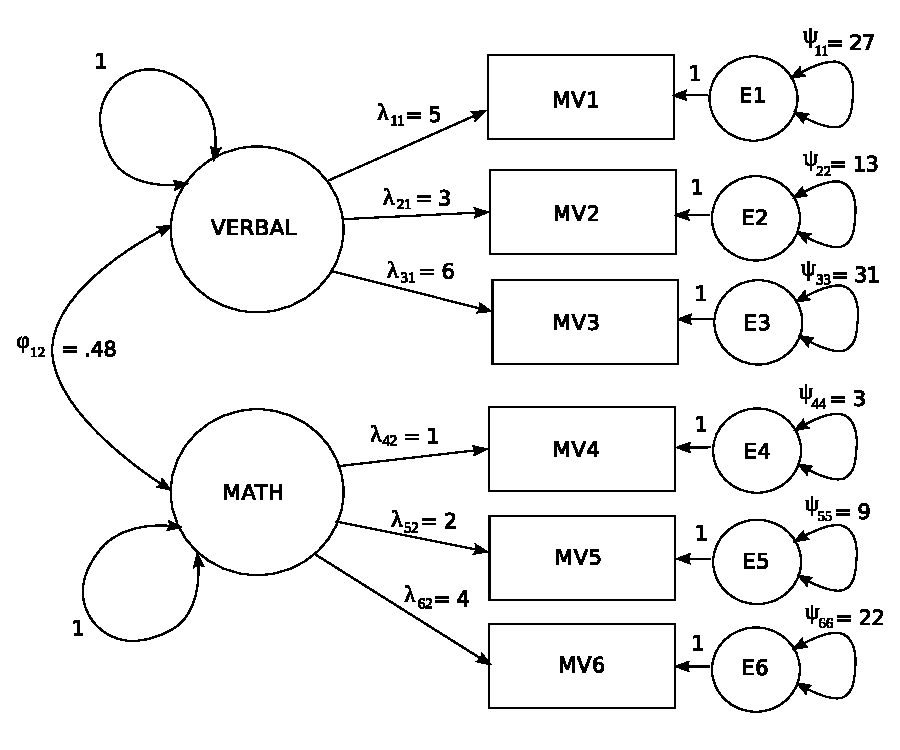
\includegraphics[height=3in]{../psychoco2012/model_under16.pdf}
  \end{center}}

\frame{
  \frametitle{Example (Age~$>$~16)}
  % path diagram illustrating parameters being the same for everyone
  \begin{center}
      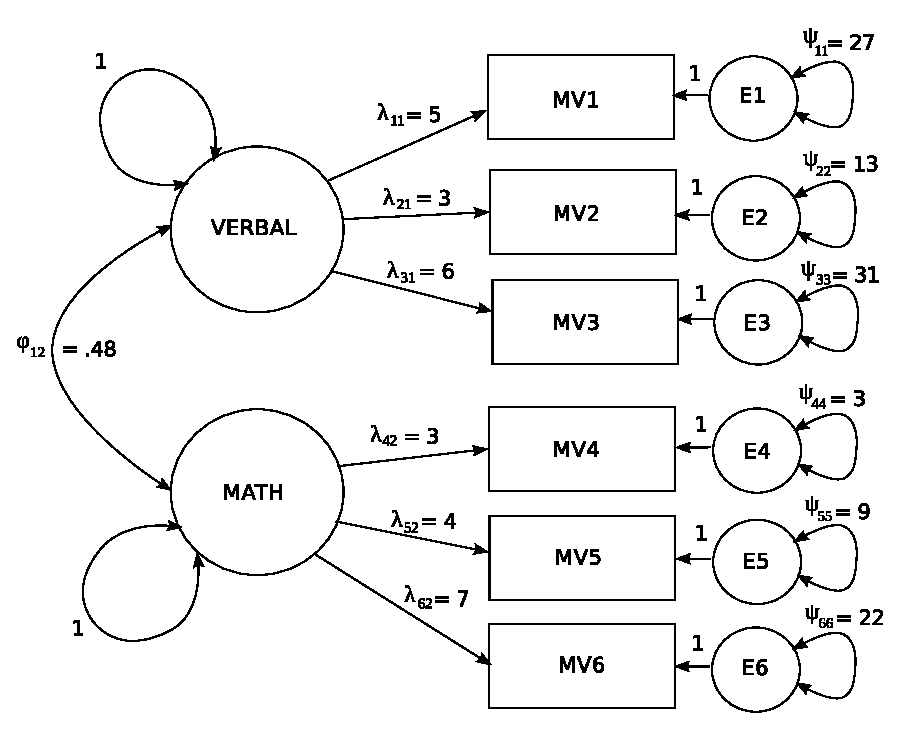
\includegraphics[height=3in]{../psychoco2012/model_over16.pdf}
  \end{center}}

% Define as theta_i = theta_0, i=1,..,n
\frame{
  \frametitle{Hypotheses}
  \begin{itemize}
    % \item There exist many types of measurement invariance,
    %   based on specific subsets of parameters being allowed
    %   to vary across individuals (e.g., Meredith, 1993).\\ \ \\
    \item Hypothesis of ``full'' measurement invariance:\\
      \begin{center}
          $H_0: \bm{\theta}_i = \bm{\theta}_0, i=1,\ldots,n$\\
          $H_1: \text{Not all the }\bm{\theta}_i = \bm{\theta}_0$
      \end{center}
      where $\bm{\theta}_i = (\lambda_{i, 1, 1}, \dots, \psi_{i, 1, 1}, \dots, \varphi_{i, 1, 2})^\top$
      is the full $p$-dimensional parameter vector for individual $i$.
  \end{itemize}}

% Too difficult to assess, so use an auxiliary variable to place
% people in meaningful groups
  % continuous vs categorical auxiliary variable
\frame{
  \frametitle{Hypotheses}
  \begin{itemize}
    \item $H_0$ from the previous slide is difficult to fully assess
      due to all the ways by which individuals may differ.\\ \ \\
    \item We typically place people into groups based on a meaningful
      auxiliary variable, then study measurement invariance across
      those groups (via Likelihood Ratio tests, Lagrange multiplier
      tests, Wald tests).\\ \ \\
    \item If we did not know the groups in advance, we could conduct
      a LR or LM test for each possible grouping, then take the maximum.
      Requires different critical values! (Can be obtained from proposed
      tests.)
  \end{itemize}}

\frame{
  \frametitle{Lack of Grouping}
  \begin{center}
      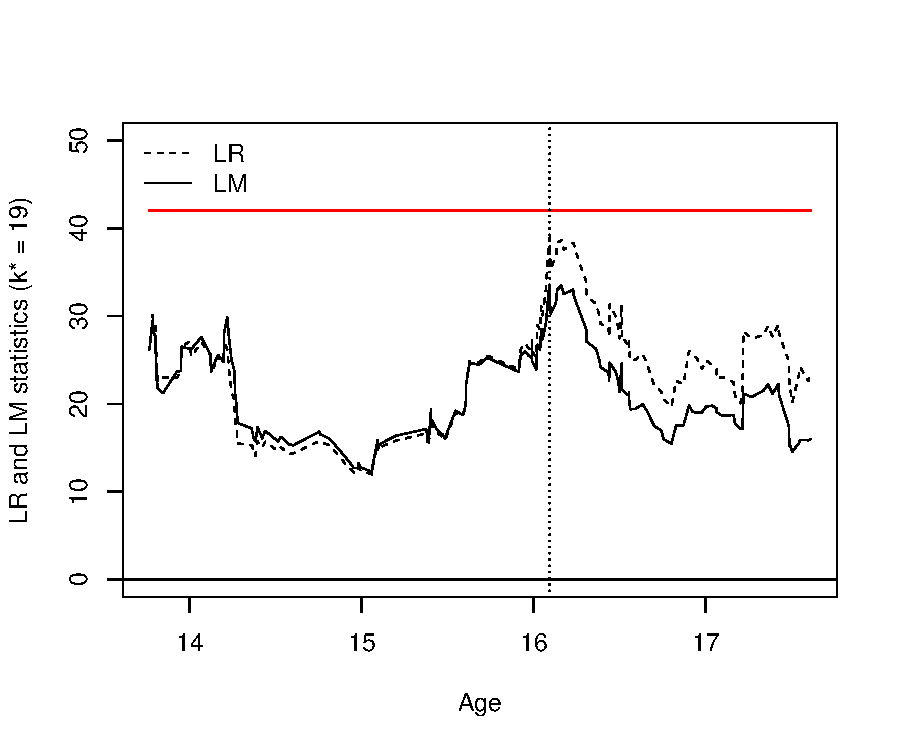
\includegraphics[height=3in]{../psychoco2012/paper-lm-lr-19.pdf}
  \end{center}
}

\section{Tests Along a Continuum}
% \frame{
%   \frametitle{Proposed Tests}
%   \begin{itemize}
%     \item In contrast to existing tests of measurement invariance, the
%       proposed tests offer the abilities to:
%       \begin{itemize}
%         \item Test for measurement invariance when groups are
%           ill-defined (e.g., when the grouping variable is continuous).
%         \item Test for measurement invariance in any subset of model
%           parameters.
%         \item Interpret the nature of measurement invariance violations.
%       \end{itemize}
%   \end{itemize}}

\frame{
  \frametitle{Proposed Tests}
  \begin{itemize}
    \item We propose a number of tests for measurement invariance
      along a continuous auxiliary variable.
    \item Tests are based on individual terms ({\em scores}) of the gradient.  The scores tell us how well a particular parameter describes a particular individual.
  % Equation of gradient vs scores for individuals
  \end{itemize}
\begin{eqnarray*}
  \displaystyle\sum_{i=1}^{n} s(\hat{\bm{\theta}} ; \bm{x}_i) =
  {\bm 0},\text{ where} \\
 \\
  s(\hat{{\bm \theta}}; \bm{x}_i) = \frac{\partial}{\partial \bm{\theta}} \log
\text{L}({\bm{x}}_i, {\bm{\theta}}) \big |_{\bm{\theta} = \widehat{\bm{\theta}}}
\end{eqnarray*}}


\frame{
  \frametitle{Proposed Tests}
  \begin{itemize}
    \item Under measurement invariance, parameter estimates should
      roughly describe everyone equally well.  So, people's scores
      should fluctuate around zero as we move up the auxiliary variable.\\ \ \\
    \item If measurement invariance is violated, the scores should
      stray from zero around specific points of the auxiliary variable.
  \end{itemize}}

\begin{frame}[fragile]
  \frametitle{Aggregating Scores}
 % define cumulative scores and other notation
  \begin{itemize}
    \item We need a way to aggregate scores across people so that we
      can draw some general conclusions.
      \begin{itemize}
        \item Order individuals by the auxiliary variable.\\ \ \\
        \item Define $t \in (1/n, n)$.
          The {\em empirical cumulative score process} is defined by:\\
  \begin{equation*}
    \bm{B}(\hat{\bm{\theta}}; t) = \frac{1}{\sqrt{n}}
    \displaystyle\sum_{i=1}^{\lfloor nt 
      \rfloor} s(\hat{\bm{\theta}} ; \bm{x}_i).
    \end{equation*}
  where $\lfloor nt \rfloor$ is the integer part of $nt$.
      \end{itemize}
  \end{itemize}
\end{frame}


\begin{frame}[fragile]
  \frametitle{Tests}
 % show that cumulative scores follow a Brownian bridge under H_0
  \begin{itemize}
    \item Under the hypothesis of
      measurement invariance, a functional central limit
      theorem holds:
  \begin{equation*}
  {\bm{I}}(\widehat{{\bm{\theta}}})^{-1/2}{\bm{B}}(\widehat{{\bm{\theta}}}; \cdot) 
\overset{d}{\rightarrow} {\bm B}^{0}(\cdot),
  \end{equation*}
 where ${\bm{I}}(\widehat{{\bm{\theta}}})$ is the observed
 information matrix and ${\bm B}^{0}(\cdot)$ is a
 $p$-dimensional Brownian bridge.\\ \ \\

   \item Testing procedure: Compute an aggregated statistic of the empirical
     score process and compare with corresponding quantile of aggregated
     Brownian motion.\\ \ \\

    \item Test statistics: Special cases include double maximum (DM), Cram\'er-von Mises
      (CvM), maximum of LM statistics.
  \end{itemize}
\end{frame}

\frame{
  \frametitle{Simulation}
  \begin{itemize}
    \item Simulation: What is the power of the proposed tests?\\ \ \\
      \begin{itemize}
        \item Two-factor model, with three indicators each.
        \item Measurement invariance violation in three factor loading parameters, with magnitude from 0--4 standard errors.
        \item Sample size in $\{100, 200, 500\}$.
        \item Model parameters tested in $\{3, 19\}$.
        \item Three test statistics.
      \end{itemize}
  \end{itemize}}

\frame{
  \frametitle{Simulation}
  \begin{center}
      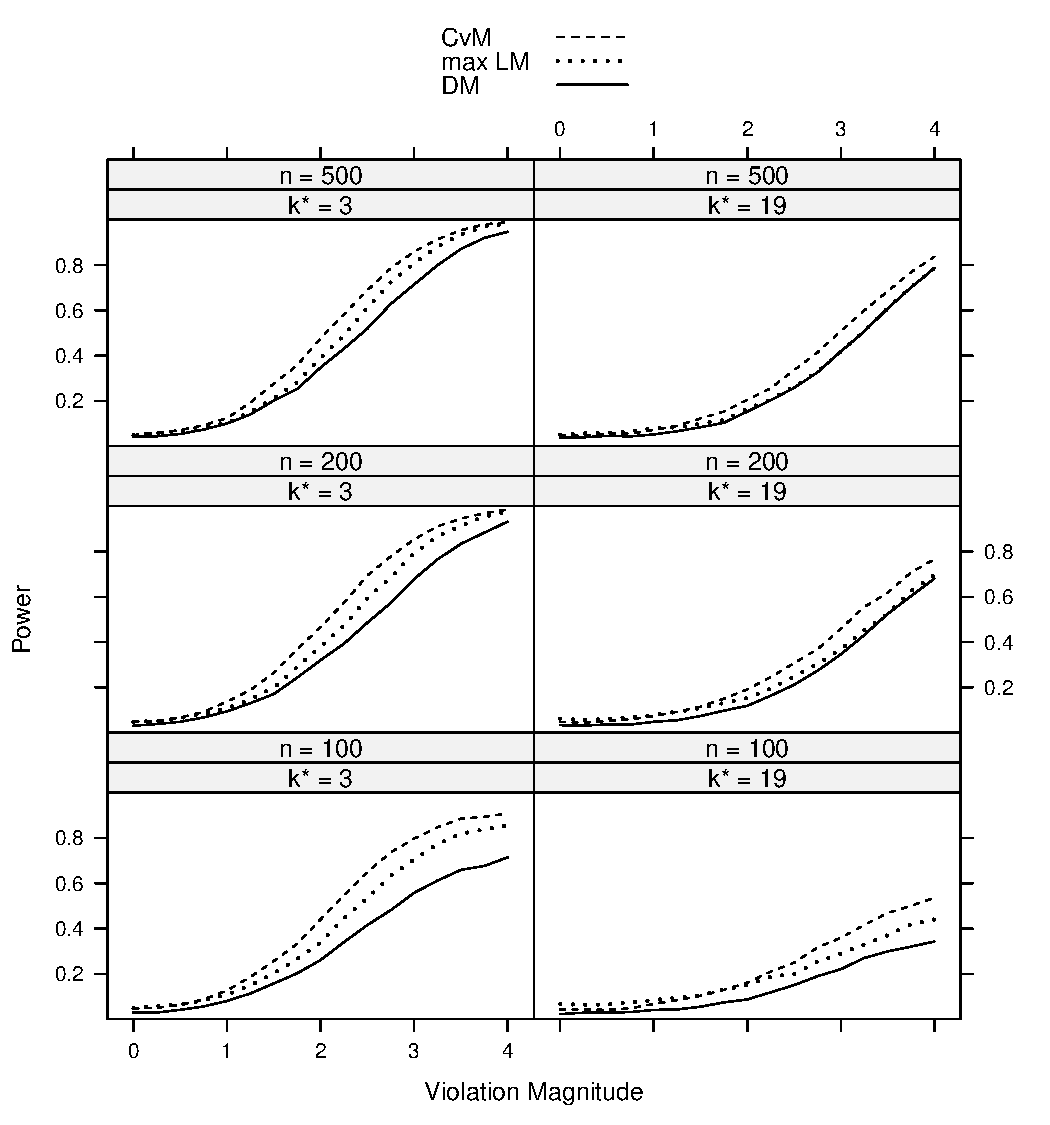
\includegraphics[height=3in]{../psychoco2012/paper-mzsim-xyplot.pdf}
  \end{center}
}

\section{Tests Along an Ordinal Variable}
\frame{
  \frametitle{Tests Along Ordinal Variables}
  \begin{itemize}
    \item The statistics described above do not immediately translate
      to ordinal auxiliary variables, where there is no unique ordering of
      individuals.
    \item To obtain a test statistic, we allow all individuals with the
      same value of the 
      auxiliary variable to simultaneously enter into the cumulative
      sum.  We then take the maximum of the cumulative sum.
    \item Critical values are obtained by summing bins of a Brownian
      bridge, where bin sizes match the observed bin sizes of the 
      ordinal variable.
  \end{itemize}}

% Achim: Can you outline ordmax and possibly ordwmax here?
\frame{
  \frametitle{Test Statistics}
}

\frame{
  \frametitle{Simulation}
  \begin{itemize}
    \item Simulation:
      \begin{itemize}
        \item Same two-factor model from before.
        \item Measurement invariance violation in three unique
          variance parameters, growing as we move up the ordinal
          variable.
        \item Sample size in $\{120, 480, 960\}$.
        \item Levels of the ordinal variable in $\{4, 8, 12\}$.
        \item Five test statistics.
      \end{itemize}
  \end{itemize}}

\frame{
  \frametitle{Simulation}
  % Graph of results
}

% Wicherts example removed due to time constraints (about 15min)

\section{Conclusions}
\frame{
  \frametitle{Conclusions}
  \begin{itemize}
    \item Measurement invariance tests utilizing stochastic processes have 
      important advantages over existing tests:
      \begin{itemize}
        \item Testing for measurement invariance along a continuum,
          defining subgroups based on the test.
        \item Testing for measurement invariance wrt an ordinal
          variable, with sensitivity to ``ordinal'' violations.
        \item Testing for measurement invariance at low $n$, where
          multiple-group models are not feasible.
      \end{itemize}
  \end{itemize}}

\frame{
  \frametitle{Software}
  \begin{itemize}
    \item We can carry out the tests for general SEMs in R, using
      \begin{itemize}
        \item \texttt{lavaan} for model estimation.
        \item \texttt{estfun()} for score extraction, which is
          currently a combination of our own code and \texttt{lavaan}
          code.
        \item \texttt{strucchange} for carrying out the proposed tests
          with the scores from \texttt{estfun()}.
      \end{itemize}
  \end{itemize}}

\frame{
  \frametitle{Current Work}
  \begin{itemize}
    \item Detailed examination of test properties.\\ \ \\
    \item Extension to related psychometric issues.\\ \ \\
    \item Continued test implementation via \texttt{strucchange} and \texttt{lavaan} (and possibly \texttt{OpenMx}).\\ \ \\
    \item Paper: Merkle, E.\ C.\ \& Zeileis, A.\ (accepted).  Tests of measurement invariance without subgroups:\ {A} generalization of classical methods.  {\em Psychometrika}.
  \end{itemize}}

\frame{
  \frametitle{}
  \begin{itemize}
  \item Questions?
  \end{itemize}}

\end{document}
